\setcounter{chapter}{5}
\setchapterabstract{This chapter outlines EU competition law enforcement and remedies, focusing on public and private mechanisms. It explains how the EU Commission and National Competition Authorities (NCAs) enforce Articles 101 and 102 to maintain fair competition. Public enforcement protects market integrity through fines and investigations, while private enforcement compensates victims and enhances deterrence. The European Competition Network coordinates case allocation, and the “Effects Principle” applies in cross-border cases. The chapter also covers leniency programs, fines, and commitment decisions as tools for compliance, and addresses enforcement challenges, proposing improvements like leniency programs and settlements to boost deterrence.}
\chapter{Enforcement and Remedies}
\vspace{-1.5cm}

{\chaptoc\noindent\begin{minipage}[inner sep=0,outer sep=0]{0.9\linewidth}\section*{Cops and Judges}\end{minipage}}

    \Example{Federico is driving but he is distracted because he is constantly checking for the number of likes he receives on his Instagram account. Thus, he crosses an intersection when the traffic light is red. This behavior is considered very dangerous and thus unlawful. It should be punished because it worsens the well functioning of a specific “market” (traffic circulation/flows). If detected, Federico will be fined (+ maybe the suspension of the driving licence) by the local police (a public body) If, in addition, Federico causes a car accident, injuring Ottavia, he will also be called to pay damages (personal and material damages to Ottavia). Usually, it is the local police that apply a fine, while a civil judge awards damages}

    \Remark{
    Why two channels?
    Because they have different (complementary) aims / purposes.
    }

    \noindent
    \textbf{Public enforcement} (usually, entrusted to public bodies- authorities) is aimed at defending a public good: the “well functioning of the market”. To this end, enforcers have two main tools:
        \begin{enumerate}
            \item \textbf{Education}, to avoid unintentional infringements;
            \item \textbf{Sanctions}, to punish those who intentionally or negligently infringe competition law. The idea is to punish and deter
        \end{enumerate}

    Nothing new: Cesare Beccaria,\textit{ On Crime and Punishments}, 1764.

    \noindent
    \textbf{Private enforcement} (judges) is aimed at compensating victims (damages). However, private enforcement also increases deterrence (because the wrongdoer must pay a fine and damages).

    \newpage
\section{Enforcers of EU Competition Law}

        \begin{itemize}
            \item \textbf{Public Enforcement System}
                \begin{itemize}
                    \item Enforced on behalf of the public to pursue the goal of maintaining a system of undistorted competition
                    \item \textbf{Public enforcers}– i.e. the EU Commission and the National Competition Authorities (NCAs), are entitled to enforce them, that is to initiate a case under art. 101/102
                \end{itemize}
            \item \textbf{Private Enforcement System}
                \begin{itemize}
                    \item Give rise to individual subjective rights that EU citizens are entitled to claim in any national court
                    \item \textbf{Private plaintiffs} can bring an action before a national court based on antitrust infringement
                \end{itemize}
        \end{itemize}

    \subsection{The enforcement model}
    
        \begin{itemize}
            \item \textbf{Goal}: to eliminate any firms’ behavior that may substantially reduce TS and CS.
            \item J\textbf{ustice perspective}: who has been harmed by wrongdoing must receive back what has been stolen to her/him.
        \end{itemize}
    
        However, enforcement is very costly. Thus, we need to contain enforcement costs or at least obtain that benefits from enforcement are greater than its costs. To achieve the first goal (extirpate wrongdoing) we must set:
    
        \begin{itemize}
            \item \(C^e > \pi^e \rightarrow \) expected cost of wrongdoing should be greater than the expected profit.
            \item \( C^e = \alpha \cdot (S+D) \rightarrow \) (S is the fine, D are damages, \(\alpha\) is the probability of getting caught). We will further elaborate this formula later on.\sn{\Note{The probability \(\alpha\) is linked to the resources invested in law enforcement. The greater are these resources + the more effective are the investigative powers \(\rightarrow\) the greater is the probability \(\alpha\) of finding a cartel.}}
        \end{itemize}

        If costs caused by enforcement activity are greater than the benefits obtained from it (in terms of avoiding any surplus reduction due to cartels or monopolization practices), than enforcement is inefficient from an economic point of view… still… it may be desirable for other reasons (e.g. avoid the spillover effects of excessive market power for democracy and other general goals pursued by the EU Treaty).

    \subsection{EU Public enforcement}

        Articles 101 and 102 are enforced by EU Commission and the National Competition Authorities of the 27 European Member States (MS) (Reg. 1/2003 on the application of Artt. 101 \& 102). Altogether, they form the European Competition Network (ECN), which has been established as a forum for discussion and cooperation. The ECN should ensure uniform application of EU competition rules, as well as an efficient division of work. 
        
        Within the ECN, the EU Commission and NCAs cooperate with each other by:

        \begin{itemize}
            \item \textbf{informing} each other of new cases and envisaged enforcement decisions;
            \item \textbf{coordinating} and helping each other with investigations (and from now on fine collection), where necessary;
            \item exchanging evidence and other information; and
            \item discussing various issues of common interest.
        \end{itemize}

        \subsubsection{ECN case allocation}

            Within the ECN, the authority in charge is usually the one which has received the material complaint, or the one having started the ex officio procedure… unless the case at stake affects competition in more than 3 MS or is really new. In these two latter circumstances, the Commission should advocate the case for itself. Several principles and case allocation mechanisms are considered by the Commission Notice on cooperation within the Network of Competition Authorities\sn{\Note{Not always satisfactory: see for example the FBA Amazon saga, where the EU Commission only partially avoked the case and left jurisdiction to the Italian NCA for the Italian market. Many lawsuits, different decisions, different remedies.}} (2004/C 101/03) (\href{https://eur-lex.europa.eu/legal-content/EN/TXT/HTML/?uri=CELEX:52004XC0427(02)&from=EN}{Text with EEA relevance})

            

    \subsection{The EU Commission}

        The EU Commission represents and upholds the interests of the EU as a whole. It does not only enforce EU law (i.e. investigate and decide), but also proposes new laws (directives and regulations) to Parliament and Council as well as second-order legislations (soft law: guidelines, guidance, notices, etc.). Within the Commission, the DG competition (DG-COMP) is the branch that starts antitrust actions against companies, while the final decision is taken by the EU Commission itself.

            \Remark{The 27 commissioners take the final decision, while the DG competition acts like a prosecutor (pressing charges, but also proposing the final decision; almost never changed by the other Commissioners)}

        Within the DG competition, the Chief Economist assists in evaluating the economic impact of business practices; other C\&B.\sn{\Note{Prosecutorial bias (and, again, political bias? Comm. Vestager was also in charge of digital; the new Comm. Ribeira will be in charge of both competition and clean and just transition (green deal, etc. ) Technical soul 10}}

        \subsubsection{How it works?}

        \begin{figure}[h]
            \centering
            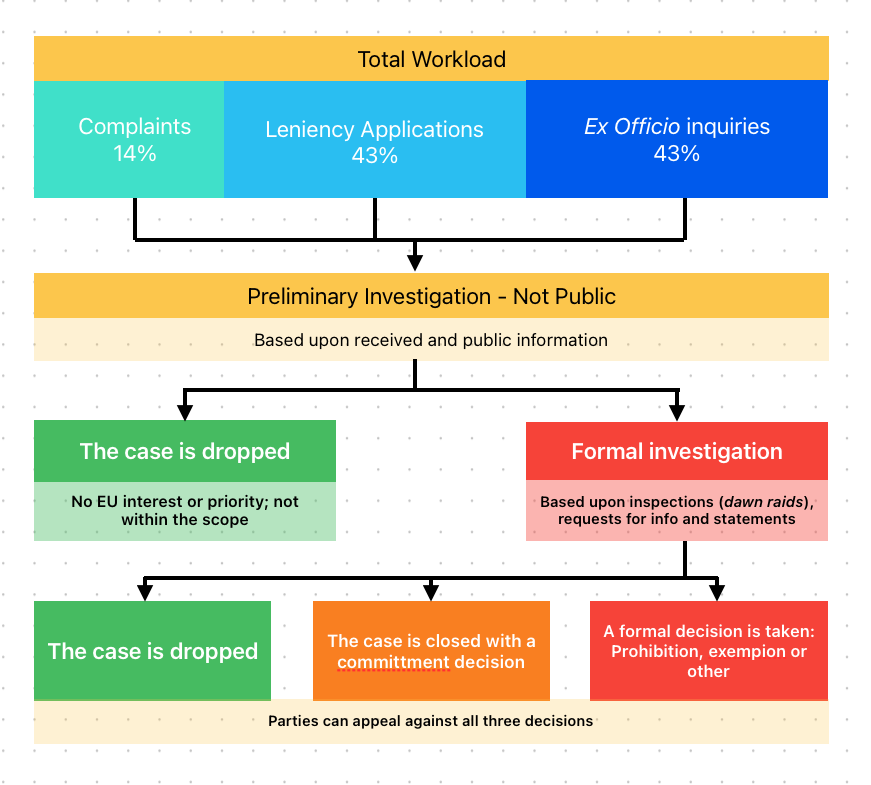
\includegraphics[width=0.50\linewidth]{TotalWorkload.png}
        \end{figure}

\section{The National Competition Authorities}

    According to Reg. 1/2003, all NCAs should have the powers to:
    \begin{itemize}
        \item Apply Articles 101 and 102 in individual cases;
        \item Fully Investigate (on site inspections, right to ask, right to seize documents, etc.)
        \item Act on their own initiative or on a complaint, receive leniency applications;
        \item Take decisions like those the Commission is allowed to take;
        \item Drop a case.\sn{\Note{In addition, in each MS the parties should bring appeals against NCAs decisions.}}
    \end{itemize}
    
    From 2004 till 2023, more than 90\% of all the decisions that applied EU antitrust rules were taken by NCAs. So, it's essential that NCA:
    \begin{enumerate}
        \item Are and act independently;
        \item ave all the necessary resources (financial, human, technological)
        \item Have enough powers to effectively enforce EU competition rules.
    \end{enumerate}
    In the past, many major differences (independence, resources, powers, fines, etc.), no efficiency, no level playing field (free riding), no cooperation between authorities (e.g.: how could you ask the German officers to help you with a surprise inspection given that they did not have the right to carry out dawn raids?). 

        \subsubsection{Time for a Change}

            \Remark{ECN+ Directive, 1/2019 to empower NCA to be more effective enforcers of EC competition law rules.}

            It introduced \textbf{Minimum Standard rules} on:
            \begin{itemize}
                \item \textbf{Independence} (from governments and business) 
                \item \textbf{Resources} (skilled economists and lawyers are very “expensive”, investigations are costly, etc.). Many models. 
                \item \textbf{Investigative Powers} (on site investigation, e- investigation, data gathering and elaboration, power to search evidence also at home, etc.) 
                \item \textbf{Decisional Powers} (interim measures, commitments, prohibition decisions, behavioural and structural remedies) 
                \item \textbf{Sanctioning powers} (same kind of - very high - fines for substantive and procedural violations, same caps, etc.).
            \end{itemize}

\newpage
    \subsection{Appeal: How does it work?}

        \begin{figure}[h]
            \centering
            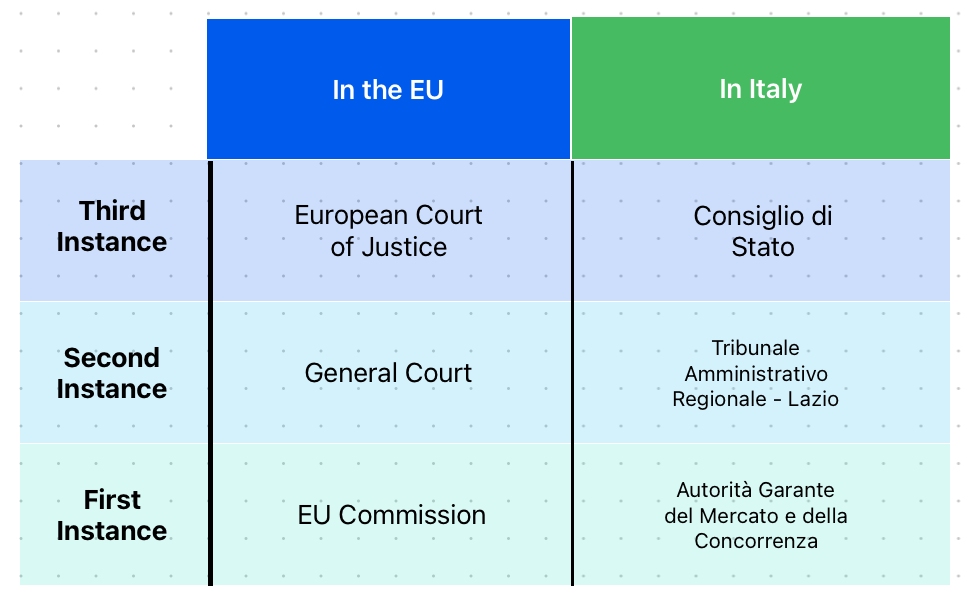
\includegraphics[width=0.65\linewidth]{appeal.png}
        \end{figure}

    \subsection{The General Court and the CJEU}

    \begin{enumerate}
        \item EU Commission decisions can be appealed in front of the EU General Court, which can confirm, amend or annul the decision for both substantive and procedural reasons. Furthermore, the Court can cancel, reduce or increase the fine imposed by the Commission.
        \item Judgments of the General Court can be appealed before the Court of Justice of the European Union (CJEU) by the unsuccessful party (the Commission can be the appellant as well)\sn{\Note{However, appeals to the CJEU are limited to questions of law (no discussion on the facts, new evidence, etc.).}}.
    \end{enumerate}

    The CJEU is the main European judicial body ensuring uniform interpretation and application of competition law across the EU. The CJEU intervenes on competition matters on two occasions:
        \begin{itemize}
            \item when an individual appeals a ruling of the General Court, to annul the judgment or
            \item when a national court refers a case, to clarify the interpretation of competition law on a specific issue.
        \end{itemize}

    \subsection{EU Competition Law Application}

        \begin{quote}
            Whoever applies EU competition law must guarantee its \textbf{uniform and effective application.}
        \end{quote}

        In other words, NCA and national Courts cannot take decisions running counter to the decisional practice of the Commission and, above all, the case law of the General Court and the CJEU. Within the ECN, the European Commission works as a: However, the CJEU is the final decision maker/interpreter\sn{\textit{Princeps inter pares}} of EU competition law.

        \Remark{True, but quite often NCAs and especially national judges do not wholly comply with EU law and do not fill the need to interpret the law in a way that is consistent with EU law and principles. What could be some ways to solve this issue?}
        
\newpage
\section{The Scope of EU Competition Law}

    EU law applies when the firm’s conduct “may affect trade between MS”.  
    If firms of more MS are involved, the practice affects trade between MS.  
    However, this rule is interpreted broadly, at least by EU enforcers and the majority of NCAs.
    \begin{itemize}
        \item Usually, a practice affects EU trade even if it only involves firms belonging to one and the same MS (e.g., France)\sn{\Note{in some MS, even local cartels have been analysed under EU law}}.
    \end{itemize}
    
    \begin{itemize}
        \item[a.] If a behaviour is conceived and impacts only non-EU citizens and territories, article 101 and 102 are not applicable (no influence on EU trade);
        \item[b.] But the “\textbf{Effects Principle}” applies. On the one hand, EU competition law can be applied beyond EU borders \textit{if} the conduct at stake produces effects on trade within the EU (an agreement by two Taiwanese firms to raise prices of goods sold in Europe); on the other hand, the Commission cannot apply EU competition law to a cartel between two European firms if the effects of this cartel are limited to China;
        \item[c.]  If the behaviour affects part of a Member State, but does not affect trade between Member States (for example, a local cartel to fix the price of olive oil in Sardinia), EU law cannot be applied. A National Competition Authority (NCA) can apply its national competition law (e.g.: the Italian competition law).
        \item[d.] What if both national law and EU law apply?
    \end{itemize}

\section{Remedies}

    \subsection{Prohibition Decisions}

        Article 7, Reg 1/2003: if, after a full investigation, the EU Commission's concerns are not– or only partly - dispelled it takes a decision: 
        \begin{itemize}
            \item[a.] forbidding the identified infringement
            \item[b.] requiring that the infringement be brought to an end (“termination”), and
            \item[c. ]usually imposing fines. 
        \end{itemize}

        Via such a decision the Commission may also:
        \begin{itemize}
            \item[d.] impose some positive/negative actions (behavioral or structural remedies), such as the duty (i) to share a proprietary input or (ii) to divest some activities and assets or (iii) to split the firm in some independent divisions (like in the Standard Oil case).
        \end{itemize}

    \subsection{Fines - Article 23 of Reg 1/2003}

        The Commission may by decision impose fines on undertakings where, either intentionally or negligently they infringe Article 101 or 102 TfUE For each undertaking (…) participating in the infringement, the fine shall not exceed 10\% of its total turnover in the preceding business year (cap or legal maximum).

        \Remark{In fixing the amount of the fine,“regard shall be had both to the GRAVITY and to the DURATION of the infringement”.}

        Other «legal» principles to be followed when fining a firm:
        \begin{itemize}
            \item \textbf{Proportionality} (linked to the specific wrongdoing, i.e. the relevant market in which the wrongdoing has been perpetrated, etc.)
            \item \textbf{Personality} (linked to the the wrongdoer, its dimensions, profits, etc.)
        \end{itemize}

        \subsubsection{Fines for Cartels}

            \begin{tabular}{|l|l|r|}
            \hline
            Year & Case name & Amount in €*) \\
            \hline
            2016/2017 & Trucks & 3 807 022 000 \\
            2012 & TV and computer monitor tubes & 1 409 588 000 \\
            2013/2016/2021 & Euro interest rates derivatives (EIRD) & 1 308 172 000 \\
            2008 & Carglass & 1 185 500 000 \\
            2019 & Forex & 1 413 274 000 \\
            2014 & Automotive bearings & 953 306 000 \\
            ++2021++ & Car emissions & 875 189 000 \\
            2007 & Elevators and escalators & 832 422 250 \\
            2001 & Vitamins & 790 515 000 \\
            2010/2017 & Airfreight (incl. re-adoption) & 785 345 000 \\
            \hline
            \end{tabular}

        \subsubsection{Monetary Fines on Firms}

            The Commission's fining policy is aimed at punishing and deterring unlawful practices. It mirrors utilitarianism, according to which, say Ce and Πe the expected costs and benefits implied by wrongdoings, economic agents are prevented from committing wrongdoings when:
            
            \begin{equation}
                C^e > \Pi^e
            \end{equation}
            
            Which is almost impossible.
            
            \Remark{\textbf{Basic Goal}: Fines should have the necessary deterrent effect on the undertaking concerned (\textbf{specific deterrence}) and should influence actual and future decisions and strategies of other undertaking (\textbf{general deterrence}).}

            In EU no fines on individuals, such as:
            \begin{itemize}
                \item  monetary fines
                \item disqualification orders
                \item imprisonment
            \end{itemize}

\newpage
            
    \subsection{Fine Quantification}

        \subsubsection{EU Guidelines on Quantification}

            \begin{itemize}
                \item \textbf{BASIC AMOUNT} (“objective” part of the quantification) = $BF + EF$
                \item \textbf{BF} = (Basic Fine)
                    \begin{enumerate}
                        \item To link the fine to the harm, BF takes into consideration the value of sale of goods/services to which the infringement relates ($\text{TURNmkt}_1$ ); multiplied by
                        \item \textbf{Gravity} = (GRAV) = (0-30\%). Various factors, such as nature of the infringement, implementation, market effects, market power of the participants. The more serious is the infringement, the higher is the percentage (almost always 30\% for covert cartels, bid rigging, etc.)
                        \item \textbf{Duration} = (DUR) = actual duration (implementation) of the infringement.
                    \end{enumerate}
                \item \textbf{EF} = (Entry Fee) = 15-25\% of TURNmkt1
                    \begin{enumerate}
                        \setcounter{enumi}{3}
                        \item EF is applied when the nature of the infringement is very serious (cartels).\sn{\Note{the goal is to deter undertakings to even try to entering into horizontal price fixing, market sharing, etc.}}
                    \end{enumerate}
            \end{itemize}

            Thus, even if duration is 0 because the cartel has not yet been implemented, EF ensure that the firms involved will receive a (heavy) fine.

        \subsubsection{Rationale of the Entry Fee}

            For very serious infringements, attempt is enough to trigger a fine, because the law tries to prevent the consummation of an illegal act. This is also typical in other fields of the law, for example in criminal law.

            Think at the following string of actions:
                \begin{enumerate}
                    \item a man threats a woman with a gun;
                    \item he opens fire;
                    \item the woman is shot to dead.
                \end{enumerate}

            To nip in the bud homicides, the law sanctions not only (3) (homicide or murder), but also (2) (attempted murder; even if the victim did not die or was not hit by the bullet), and (1) (preparatory steps with the aim of killing someone, even if the man was halted/detained before the fact).

        \subsubsection{Further Guidelines on Quantification}

            \begin{itemize}
                \item \textbf{Adjustments}
                    \begin{enumerate}
                    \setcounter{enumi}{4}
                        \item A\textbf{ggravating factors} (AGGF): obstruction, instigation, recidivism, ringleader, etc.
                        \item \textbf{Mitigating factors} (MITF): early termination, negligence, limited involvement, no implementation, cooperation, encouragement by public bodies or legislation;
                        \item Special increase for \textbf{deterrence} (DET) (the Microsoft factor– see infra\sn{\Note{2004: Microsoft profits > 9 billion USD. Initial fine = profits earned in 1 week}})
                        \item \textbf{Inability to pay}: fine reduction in some specific circumstances (high risk of market exit with “social effects” and effects on the structure of the market)\sn{\Note{The maximum fine must be capped at 10\% of the overall world annual turnover of the undertaking, which is the statutory limit.}}
                    \end{enumerate}
            \end{itemize}

            \Example{“When calculating the initial amount of the fine, account should be taken of the necessity of setting the fine at a level that ensures that it has a sufficient deterrent effect. In order to do so, it is necessary to determine whether any upward adjustment of the initial amount is necessary. Given Microsoft's significant economic capacity, in order to ensure a sufficient deterrent effect on Microsoft, the initial amount should be adjusted upwards by a factor of 2”}

            \Example{
            FYF (a) sells fruit (bananas and oranges) in EU and Asia; (b) FYF is the ringleader of a banana cartel in Germany; (c) The cartel lasted 20 years; (d) FYF has been already fined in the past for having participated to the lemons’ cartel in Italy.
            FYF world turnover is 500 million €/year (WTURN); FYF bananas turnover is 200 million €/year. FYF bananas turnover in Germany is 50 million €/year (TURNmkt1). FYF cooperated with the Commission during the investigation. How can you determine FYF’S fine in this very simple situation? \textbf{The magic formula:}
            \begin{itemize}
                \item \( S = \langle \text{BASIC AMOUNT} \rangle + \text{AGGF} - \text{MITF} + \text{DET} < S^* \)
                \item \( S = \langle (\text{GRAV} \times \text{DUR} \times \text{TURNmkt1}) + \text{EF} \rangle + \text{AGGF} - \text{MITF} + \text{DET} < S^*  \)
                \item \( S = \langle ((0 - 30\%) \times \text{DUR} \times \text{TURNmkt}_1) + (15 - 25\%) \times \text{TURNmkt}_1 \rangle + \text{AGGF} - \text{MITF} + \text{DET} < S^* \)
                \item \( S = \langle 0.3 \times 20 \times 50 + 0.25 \times 50 \rangle + (40 + 30) - 10 + 0 = 372.5 \)
                \item \( \text{However, } S^* = 10\% \times \text{WTURN} = 0.1 \times 500 = 50 \)
            \end{itemize}
            \[ S > S^* \text{ then } S = S^* = 50 \]
            }

    \subsection{Deterrence - Optimal fining - ex ante v. ex post}

        Are monetary fines enough to deter cartels ? Consider Z, a mono-product firm carrying out business in France. Hypothesis: Profits derived from entering a cartel amount to 10\% of Z turnover (T) each year. If you want to deter, fines should be set to encourage Z not to enter the cartel, i.e., from an ex-ante perspective: don’t even dare to try!

        Thus, let’s consider the moment in which Z has to choose if entering a cartel. Z will weigh the expected profits and the expected costs deriving from entering entering the cartel.
        \[ \Pi^e > C^e \]
        then Z will choose to participate to the wrongdoing. On the contrary, if \( \Pi^e< C^e\) , it will turn down the proposal.

\newpage
        The formula for $C^e$ is equal to
        \begin{equation}
            C^e = a \cdot b \cdot \frac{S+D}{q}
        \end{equation}
        Where
        \begin{itemize}
            \item $S$ = Fines (in the EU, max 10\%T);
            \item $D$ = Damages
            \item $a < 1$ = is the probability to detect a suspect behaviour;
            \item $b < 1$ = is the probability to find enough evidence about that behaviour;
            \item $q \geq 1$ = is the quashed/annulment factor.
                \begin{itemize}
                    \item If \( q = 1 \), it means that courts never reverse a NCA’s decision;
                    \item If, \(q > 1\), it means that courts at least sometimes reverse NCA’s decisions, and/or reduce the amount of the fine $S$.
                \end{itemize}
            \item 
        \end{itemize}

        \subsubsection{A numerical example}

        Let's consider a 1-year framework and suppose that: $\pi_e = 10\%T$; $q$ is 2 (on average 1 out of 2 decisions is reversed by a higher court); the joint probability \(a \cdot b\) is roughly 15\%.

        Thus, even if $S = S^* = 10\%.T$, and $D = \pi^e = 10\%.T$,
        the expected cost of participating to a cartel is $0.075.(0.1T+0.1T) = 0.015.T$
        
        The longer is the cartel before being detected and terminated, the greater are the
        expected gains of a cartel. For example, after 3 years:
        
        $\pi^e = 0.3.T$, while expected costs are: $0.075 (0.1+0.3T) = 0.03T$.
        
        In countries where $D$ are not fully compensated, this difference may be really huge: after 1 year $\pi^e = 0,1T$, while $C^e = 0,015 T$, i.e., expected profits are 8 times larger than expected costs. And the difference grows overtime: After 3 years, expected profits are 10 times larger than expected costs.
        
        \subsubsection{And now, what can we do?}

            How can we improve deterrence, i.e. the expected cost of wrongdoing?

            \begin{enumerate}
                \item improving «D» and «S»? Possible, but limited: ex post a/all firm/s could fail if S and D are too high (other fines? Criminal fines may deter more, but it is also more difficult to prove infringements because of the standards of evaluation ...);
                \item Improving the solidity of competition authorities’ decision, i.e., decreasing the quash factor “q”? Possible, but again to a limited extent (you can educate judges - and competition authorities’ officers - this will increase the quality of decisions and judgments, and in turn this may lead to a reduced number of decisions that are quashed; however, also education is costly);
                \item improving “a” and “b”? Possible, but subject to budget constraints (if you increase the number of phd in economics working on detecting cartels, you must fire lawyers that collect evidence and take care of the investigation).
            \end{enumerate}

        \subsubsection{Ways out}

            \begin{enumerate}
                \item (i) Increasing «a.b» (i.e., joint probability to detect and to prove an infringement), without increasing the budget, using amnesty/leniency programs). Creating a sort of virtuous circle: 
                \begin{itemize}
                    \item[\(\rightarrow\)] you invest on «a», bettering detecting \& investigation techniques and thus breathing down firms’ back; 
                    \item[\(\rightarrow\)] someone in one of the firms gets scared, and thus
                    \item[\(\rightarrow\)]the firm files a request for amnesty/leniency, thus producing the evidence the Authority needs to condemn all the parties (thus, $\uparrow a \rightarrow b= 1$ ).\sn{\Note{in the EU, no criminal fines}}
                \end{itemize}
                \item Reducing the number of appeals by offering a discount on the otherwise applicable fine iff (\(\iff\)) parties admit their wrongdoing (\textbf{settlements procedure}). In that circumstance, the parties will lose interest in appealing the decision, and thus the total number of NCAs quashed decisions will decrease accordingly, i.e., it’s like reducing the quashing factor «q».
                \item Save resources by closing investigations on less serious infringements by «agreeing» with the parties a remedy that will solve the alleged competitive problem (\textbf{commitments}). Thus, you can use your resources for more serious infringements.
            \end{enumerate}

\section{EU Leniency Programme}

    Under the Commission's Leniency Program, the first firm to submit evidence of a cartel that is sufficient to either:
        \begin{itemize}
            \item launch an inspection (dawn raid) or
            \item enable the Commission to find an infringement
        \end{itemize}
    receives full exemption from fine (total immunity).
    
    In all cases, the firm must also
        \begin{enumerate}
            \item fully cooperate with the Commission throughout its procedure,
            \item provide it with all evidence in its possession, and
            \item put an end to the infringement immediately.
        \end{enumerate}
    
    Cooperation with the Commission implies that the existence and the content of the application for immunity/leniency cannot be disclosed to any other company.
    
    The company may not benefit from immunity if it took steps to coerce other undertakings to participate in the cartel.\sn{\Note{Leniency available only for secret cartels}}

    \begin{itemize}
        \item Firms not qualifying for immunity may still benefit from a reduction of fines if they provide ``significant added value'' evidence to the Commission and terminate their participation in the cartel.
        \item ``\textbf{Significant added value}'' = info that reinforces the Commission's ability to prove the infringement.
        \item The first firm to meet these conditions is granted a 30 to 50\% reduction, the second 20 to 30\%, and subsequent companies up to 20\%.
    \end{itemize}
    
    EU Leniency program is thought to:
    
    \begin{itemize}
        \item Give enforcers notice and evidence of cartels;
        \item Make cartels more unstable by incentivising cheating;
        \item Increase deterrence by increasing the probability of detecting and proving the existence of cartels;
    \end{itemize}

    \Remark{Almost all the cartels fined by the EU Commission have been brought to the attention of the Commission by a leniency application.}

    However, while it is true that $S = 0$, firms will very likely have to pay for $D$. So, why are they going to self confess if \(a \cdot b\) is low ?
    \begin{itemize}
        \item Imported leniency program application;
        \item Unstable cartels (run before it’s too late)\sn{\Note{Of course, lack of trust may depend on internal tensions, changing markets, innovation, but also efforts by the competition authorities (\textit{ex officio} proceedings, market investigations, etc.)}}; 
        \item Strategic leniency;
        \item Fear of whistleblowers;
        \item Change of control;
        \item Fear of super $S$ if the firm operates on many markets and is already a recidivist.
    \end{itemize}

    \subsection{Settlements}

    In cartel cases, the parties may propose a settlement, which the Commission may accept or reject.

    \begin{itemize}
        \item With the statement of objections, the Commission presents the parties with the evidence and notifies them of its conclusions as to duration, seriousness, liability, and likely fine.
        \item If willing to settle, the parties must make a submission acknowledging their liability and stating that they accept the Commission's statement of objections.
        \item If a settlement is reached, the parties benefit from a faster procedure and a reduction of up to 10\% of the fine.
        \item The settlement procedure allows the Commission to adopt a faster, more streamlined decision to allocate resources to other cases. In addition, given the ``confession'' of the parties, it avoids follow-on appeals on the existence of the infringement and on the firm's participation in it.
    \end{itemize}

\newpage
    \Example{
    \textbf{EU Commission fines ethylene purchasers €260 mi. in cartel settlement (2020):}
    The Commission has fined Orbia, Clariant and Celanese a total of €260 million for breaching EU antitrust rules. Westlake received full immunity for revealing the cartel, thereby avoiding an aggregate fine of ca. €190 million. Orbia, Clariant and Celanese benefited from reductions of their fines for their cooperation with the Commission investigation. The reductions reflect the timing of their cooperation and the extent to which the evidence they provided helped the Commission to prove the existence of the cartel in which they were involved. In addition, under the 2008 Settlement Notice, the Commission applied a reduction of 10\% to the fines imposed on the companies in view of their acknowledgement of the participation in the cartel and of the liability in this respect. The breakdown of the fines imposed on each company is as follows:
    }

    \begin{tabular}{|>{\raggedright\arraybackslash}m{3cm}|>{\centering\arraybackslash}m{3cm}|>{\centering\arraybackslash}m{3cm}|>{\centering\arraybackslash}m{4cm}|}
    \hline
    \textbf{Purchaser (group)} & \textbf{Reduction under Leniency Notice} & \textbf{Reduction under Settlement Notice} & \textbf{Fine (€)} \\ 
    \hline
    Westlake & 100\% & 10\% & 0 \\ 
    \hline
    Orbia & 45\% & 10\% & 22 367 000 \\ 
    \hline
    Clariant & 30\% & 10\% & 155 769 000 \\ 
    \hline
    Celanese & 20\% & 10\% & 82 307 000 \\ 
    \hline
    \end{tabular}

    \vspace{0.3cm}

    Some questions for you:
    \begin{itemize}
        \item Is a reduction of 10\% of the fine enough?
        \item Which are the overt and hidden pros \& cons of settlements?
    \end{itemize}

    \subsubsection{Recap}

    \begin{tabular}{|>{\raggedright\arraybackslash}m{4cm}|>{\raggedright\arraybackslash}m{4cm}|>{\raggedright\arraybackslash}m{4cm}|>{\raggedright\arraybackslash}m{4cm}|}
    \hline
    \textbf{Basic fine} & \textbf{Increased by} & \textbf{Decreased by} & \textbf{Subject to overall cap} \\ 
    \hline
    Percentage of value of relevant sales (0-30\%) & \textbf{Aggravating factors} & \textbf{Mitigating factors} & 10\% of global turnover (per infringement) \\ 
    \hline
    x Duration (years or periods less than one year) & e.g. ringleader, repeat offender or obstructing investigation & e.g. limited role or conduct encouraged by legislation, cooperation &  \\ 
    \hline
    + cartels 15-25\% of value of relevant sales: additional deterrence for & & &  \\ 
    \hline
    \end{tabular}

    \vspace{0.3cm}

    The fine is possibly further decreased by:
    \begin{itemize}
        \item \textbf{Leniency}: 100\% for first applicant, up to 50\% for next, 20-30\% for third and up to 20\% for others
        \item \textbf{Settlement}: 10\%
        \item \textbf{Inability to pay reduction}
    \end{itemize}

\newpage
    \subsection{Commitment Decisions}

    Antitrust decisions are very burdensome. It takes a lot of time to investigate, gather evidence, hear all the parties involved, conduct market studies, let the parties exercise their rights of defence, let their economic consultant present very complicated models, empirical studies, etc. In some circumstances, a decision with full ascertainment of facts may take more than 5 years!, and an incredible amount of resources and money both for the Commission and the parties involved.\sn{\Note{Google Shopping: probes allegations, Nov. 2010; final decision, June 2017 (and then General Court and ECJ: September 2024).}}

    \Remark{\textbf{Are those efforts always warranted?} In some circumstances C.D. are a quick alternative to decisions with full ascertainment of facts.}

    A Commitment Decision (C.D.) allows the Commission to restore effective competition without developing a full investigation into the existence of a possible antitrust infringement. Namely, with a commitment decision:

    \begin{enumerate}
        \item The Commission voices its competition concerns;
        \item The parties—usually, at a very early stage of the investigation—come forward with commitments to address these concerns;
        \item If the Commission, after consulting market participants (MARKET TEST), finds these commitments sufficient to restore effective competition, it takes a decision to make them legally binding.
    \end{enumerate}
    
    Thus, with a C.D.:
    
    \begin{itemize}
        \item The Commission may accomplish its mission of preserving markets' well functioning, saving time and resources, because it avoids a full assessment of the evidence gathered;
        \item The parties are not convicted and, hence, do not run the risk of suffering fines, follow-on civil actions, and bad reputation;
        \item In some markets, C.D.s are a very effective tool, because they allow the Commission to remedy a behaviour before it produces structural and/or irreversible negative effects.
    \end{itemize}

    \noindent Commitments decisions are not applicable when the competitive concerns regard the existence of a serious infringement (cartels, exclusionary practices);

    \begin{itemize}
        \item Commitments are usually in place for a specific period of time, and if companies breach them, they can be fined (up to 10\% of the aggregate world turnover of a company);
        \item May commitments decisions transform the nature of the antitrust authorities? Regulation?
        \item Transparency (bargaining between the parties and the Commission, no decisions on important issues, no information on doubtful behaviour).
    \end{itemize}

\newpage
\section{EU Private Enforcement}

    \begin{itemize}
        \item \textbf{1974}: CJEU, \textit{Brt v. Sabam}: The Treaty provisions on competition have direct effect, i.e., individuals can derive rights directly from those provisions, and they can invoke them before national courts.
        \item \textbf{2001}: CJEU, \textit{Courage \& Others}: Direct effect means that anyone who has suffered harm because of an infringement of competition rules is entitled to claim compensation for that harm before a national court: 
        \begin{quote}
        ``The practical effect of the prohibition laid down in Article [101] would be put at risk if it were not open to any individual to claim damages for loss caused to him by a contract or by conduct liable to restrict or distort competition.''
        \end{quote}
        \item \textbf{2004}: Article 6 of Regulation 1/2003 recognises that national courts have the power to fully apply Articles 101 and 102 (including interim measures, voidness, and compensation/damages).
    \end{itemize}

    \noindent If a plaintiff shows that there has been: (a) an antitrust infringement; and (b) that infringement caused a direct/indirect harm to her/her business, she is entitled to act and ask for compensation of the damages suffered. The onus of proof is on the plaintiff. Very difficult to prove (a), but also (b); furthermore, quantification of the harm may also be difficult.

    \begin{itemize}
        \item A plaintiff can either directly bring an action for damages in front of a court (\textit{stand-alone actions}), or
        \item Ask first (and/or wait for) the EU Commission to take a decision and then start private litigation (\textit{follow-on actions}).
    \end{itemize}
    
    \noindent The second route is by far more lengthy and feasible only in a handful of cases. Still, it has many advantages from a procedural point of view. Regulation 1/2003 states that a decision of the Commission is deemed to be irrefutably established for the purposes of proving the infringement in an action for damages brought before a national court under Article 101 or Article 102.

    \subsection{Relevance of Private enforcement (PE)}

        \noindent Why is private enforcement so important? And why should we need more private enforcement in the EU?

        \begin{enumerate}
            \item \textbf{Justice.} It gives back to consumers what firms have "stolen" by putting into effect restrictive practices and abuses of dominance (Consumer Surplus, not the Deadweight Loss);
            \item \textbf{Deterrence.} Damages (and the consequences of voidness) add up to fines. Thus, private enforcement raises the actual and expected cost of wrongdoing;
            \item \textbf{Effectiveness.} The Commission and the National Competition Authorities (NCA) can investigate only a limited number of cases. Thus, private enforcement strengthens the possibilities for complainants to seek and obtain effective relief before national courts. If the NCA cannot or is not willing to investigate, there is another channel through which it is possible to block antitrust infringements. This, in turn, increases deterrence.
        \end{enumerate}

        To boost private enforcement and actions for damages, Directive 2014/104/EU on Antitrust Damages Actions mandated national legislators to introduce some changes in national civil procedure provisions. Because of these changes, now actions are:

        \begin{itemize}
            \item \textbf{Easier:} If a National Competition Authority (NCA), not only the EU Commission, has taken an infringement decision regarding the behaviour at stake, the final infringement decision will constitute full proof before civil courts in the same Member State\sn{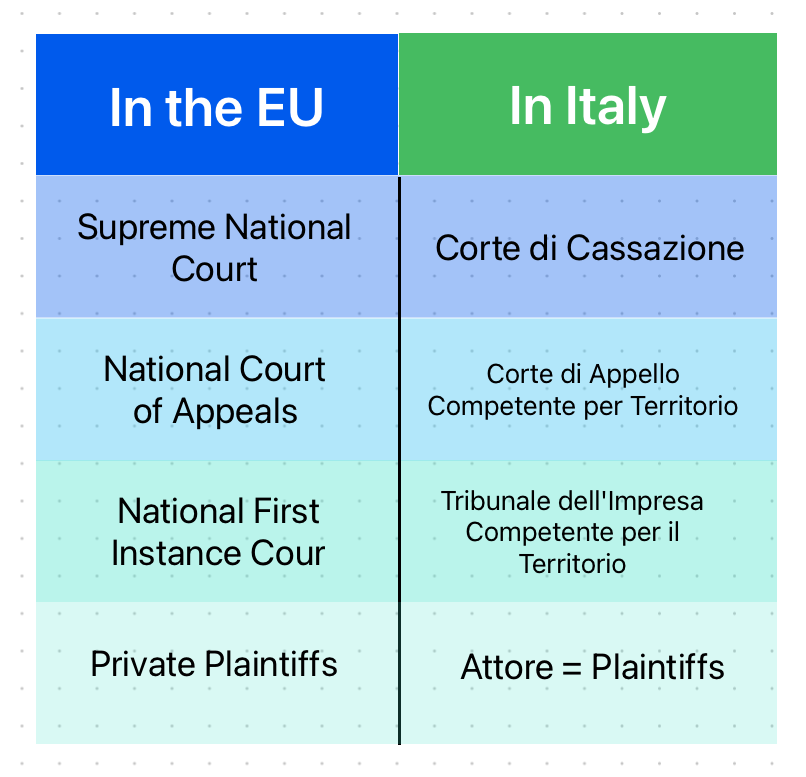
\includegraphics[width=1\linewidth]{Private_enforcement2.png}} (MS) where the infringement occurred.
            \item \textbf{Easier:} Courts can order disclosure of evidence to help victims of antitrust damages (proportionality and protection of confidential information principles apply; a big problem with leniency?).
            \item \textbf{Wider:} Indirect purchasers can bring an action for damages (contrary to the U.S.A.). Thus, if there is a cartel between producers to raise sell-in prices, and as a consequence, distributors (\textit{direct purchasers}) increase sell-out prices (or retail prices), consumers (\textit{indirect purchasers}) can also bring an action against cartelists.
        \end{itemize}

        \subsubsection{C’est domage}

            The EU Directive on damages is very important also because:

            \begin{enumerate}
                \item It establishes a (rebuttable) presumption that cartels cause harm. This will facilitate compensation, given that victims often have difficulty in proving the harm they have suffered.
                \item Calculating damages can be difficult. The Commission adopted a Communication on quantifying harm in antitrust damages actions to help national courts and parties involved in actions for damages, by explaining how to quantify the harm caused by antitrust infringements.
                \item The Directive clarifies that victims are entitled to full compensation for the harm suffered, which covers compensation for actual loss and for loss of profit, plus payment of interest from the time the harm occurred until compensation is paid.
                \item Any participant in an infringement will be responsible towards the victims for the whole harm caused by the infringement (joint and several liability), with some exceptions (e.g., for SMEs and for leniency applicants).
            \end{enumerate}
            
            \noindent Would it be wise to encourage even more action by the victims? How? What are the potential dangers in doing so?

\newpage
    \subsection{Trucks in Spain}

        \Example{
            \noindent The EU Commission found a cartel in the truck sector and fined the parties for a total of €2,926,499,000. The cartel lasted for 14 years and involved all the main European producers. They colluded on truck pricing and on passing on the costs of compliance with stricter emission rules. Thus, many acquirers were harmed, even if the EU Commission did not estimate the impact of the cartel on the final price of trucks (the agreement was prohibited by object).
            \begin{itemize}
                \item «Consumers» are transportation companies, small carriers, businesses that have fleets of trucks to distribute their products.
                \item Given the average lifespan of a truck, it means that consumers need to buy from 5 to 10\% of new trucks each year.
                \item The cartel lasted for 14 years. A firm with 100 trucks, during that period, has bought between 70 to 140 new trucks.
                \item The price of a new truck is between €80,000 to €250,000.
                \item If the overcharge due to the cartel is 10\% of the final price, then it means that for each new truck, a firm may have paid €15,000 more than the competitive price.
                \item Thus, damages amount to €1,500,000 (plus interest rates).
            \end{itemize}
            \noindent There is an incentive to ask a Court to award damages because, in case of success, the level of compensation will be greater than the costs of the (follow-on) legal action. And success is very likely too! (The illegal behaviour is proved by the EU Commission decision; harm is presumed, etc.) \\
            \noindent \textbf{Spain as a case study (updated to November 2022):}
            \noindent The result is the following (thanks to Francisco Marcos for the info):
            \begin{itemize}
                \item More than 3000 first instance judgements;
                \item 1130 Appeals judgements, 93\% favor the plaintiff (at least in part);
                \item Half of favourable judgements award damages equal to 5\% of the truck purchase price (+interest);
                \item More than a quarter of favourable judgements fully accept the plaintiff's damages quantification (average approximately 16\% of the purchase price + interest);
                \item The rest of the judgements introduce variations (either reducing what the claimant sought or using a judicial estimation of harm of 8\% or 10\%).
            \end{itemize}
        }
        